\documentclass{beamer}
\usepackage{graphicx}

\usetheme{Antibes}
\usecolortheme{crane}

\AtBeginSection[]
{
  \setcounter{tocdepth}{2}
  \begin{frame}<beamer>
    % \frametitle{Outline for section \thesection}
    \tableofcontents[currentsection, hideallsubsubsections]
  \end{frame}
  \setcounter{tocdepth}{3}
}

\title[Bees?]{``Bees?''\\ A Large Scale, Co-operative Simulation Weighing 
              Altruism and Selfishness}
\author{A. Simms, R. Thielstrom}
\institute{Swarthmore College}
\date{Adaptive Robotics, Spring 2014}


\begin{document}
  
  \begin{frame}[t]
    \titlepage
  \end{frame}


  \begin{frame}[t]\frametitle{Presentation Roadmap}
    \setcounter{tocdepth}{2}
    \tableofcontents
    \setcounter{tocdepth}{3}
  \end{frame}

  \section{Overview} % (fold)
  \label{sec:overview}

    \begin{frame}[c]\frametitle{Abstract}
      \begin{itemize}
        \item Attempting to investigate conditions for selfishness and altruism
              in a community of neural-net agents.
        \item Can we get co-operation from a large number of independent 
              agents?
      \end{itemize}
    \end{frame}

    \subsection{Model} % (fold)
    \label{sub:model}
      
      \begin{frame}[c]\frametitle{The Bee model}
        \begin{itemize}
          \item Many individual ``bees'' in a ``hive''.
          \item Each bee is an individual NEAT agent.
        \end{itemize}
      \end{frame}

    \begin{frame}[c]\frametitle{A day in the life of a bee}
      Every ``day'' in the simulation:
      \begin{itemize}
        \item Each bee goes out to get ``nectar''
        \item Has the decision to eat the nectar there, or bring it 
              back to the hive
        \item At the hive, the nectar brought back by the bees is 
              shared equally between the bees that brought back nectar.
      \end{itemize}
      Fitness is determined by the average nectar that a bee accumulates
      throughout its lifetime.
    \end{frame}

    % subsection model (end)

  % section overview (end)

  \section{Experiments} % (fold)
  \label{sec:experiments}
    \subsection{Hypothesis} % (fold)
    \label{sub:hypothesis}

      \begin{frame}[c]\frametitle{Hypothesis}
          
          The amount of altruism and selfishness demonstrated in NEAT-trained
          agents will be most affected by an individual fitness relying
          on overall group fitness.
      
      \end{frame}
    
    % subsection hypothesis (end)

    \subsection{Basic Experiments} % (fold)
    \label{sub:basic_experiments}
    
      \subsubsection{Methods} % (fold)
      \label{ssub:methods}
      
        \begin{frame}[c]\frametitle{Methods of the Basic Experiment}
          Every ``day'' in the simulation:
          \begin{itemize}
            \item Each bee goes out to get ``nectar''
            \item Has the decision to eat the nectar there, or bring it 
                  back to the hive
            \item At the hive, the nectar brought back by the bees is 
                  shared equally between the bees that brought back nectar.
            \end{itemize}
            One ``day'' is one NEAT generation.
        
        \end{frame}

      % subsubsection methods (end)

      \subsubsection{Results} % (fold)
      \label{ssub:results}

        \begin{frame}[t]\frametitle{Composition of the Hive Over Time}
          \begin{figure}
          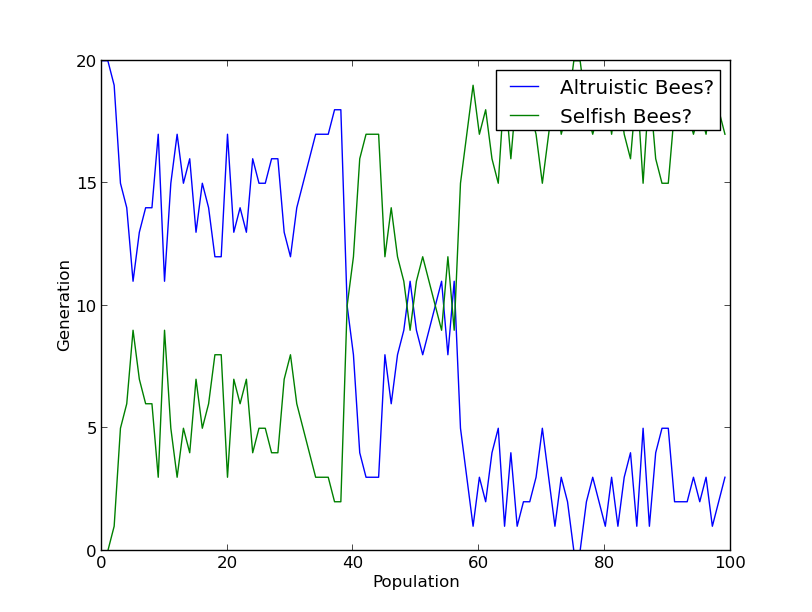
\includegraphics[width=8cm]{s_bees.png}
          \end{figure}
        \end{frame}
      
      % subsubsection results (end)

      \subsubsection{Discussion} % (fold)
      \label{ssub:discussion}
        \begin{frame}[c]\frametitle{Why are the bees selfish?}
            
          \begin{itemize}
            \item There is no substantial reason for them to cooperate.
            \item Insurance is only effective if there are a large number of
                  people paying into it.
          \end{itemize}
        
        \end{frame}
      % subsubsection discussion (end)
    % subsection basic_experiments (end)

    \subsection{Hive Fitness} % (fold)
    \label{sub:hive_fitness}
      \subsubsection{Methods} % (fold)
      \label{ssub:methods}
        \begin{frame}{Added notion of ``Hive'' fitness}
          \begin{itemize}
            \item The hive has some ``nectar reserves''.
            \item Maintained by taking some nectar from the bees that brought 
                  back nectar.
            \item A penalty is assessed to the fitness of all bees if nectar 
                  drops below a certain level.
          \end{itemize}
        \end{frame}
      % subsubsection methods (end)

      \subsubsection{Results} % (fold)
      \label{ssub:results}

        \begin{frame}[t]\frametitle{The Only Difference is Hive Fitness}
          \begin{figure}
          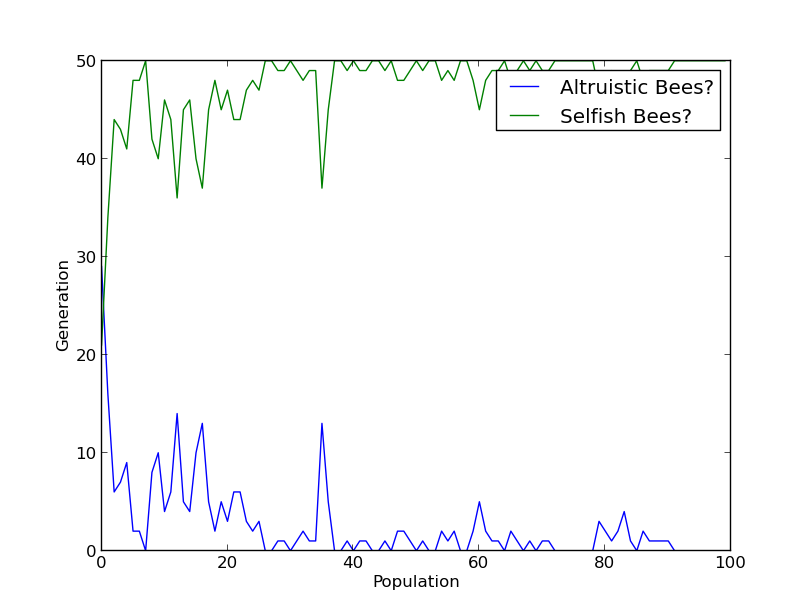
\includegraphics[width=8cm]{hive_influenced_bees.png}
          \end{figure}
        \end{frame}

        \begin{frame}[t]\frametitle{Nectar Reserves Over Time}
          \begin{figure}
          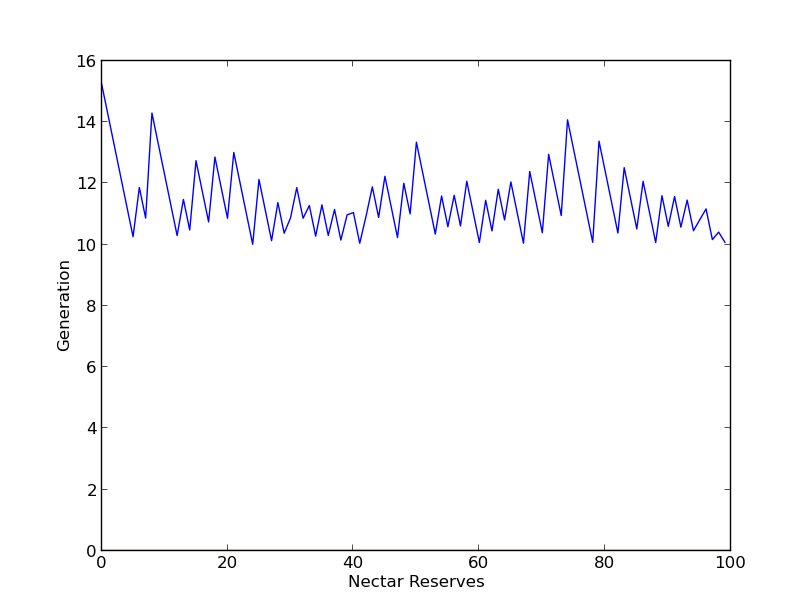
\includegraphics[width=8cm]{hive_influenced_bees_nectar.png}
          \end{figure}
        \end{frame}

      % subsubsection results (end)

      \subsubsection{Discussion} % (fold)
      \label{ssub:discussion}

        \begin{frame}[c]\frametitle{Why are the bees still selfish?}

          \begin{itemize}
            \item 0.005 is still better than 0.001
            \item Insurance only works if there are a large number of people
                  paying in
          \end{itemize}
        
        \end{frame}
      % subsubsection discussion (end)

    % subsection hive_fitness (end)

    \subsection{Recurrent Experiment} % (fold)
    \label{sub:recurrent_experiment}
    
      \begin{frame}[c]\frametitle{Rationale}
        \begin{itemize}
          \item Bees live more than one day, why shouldn't our simulated bees?
          \item Drawing inspiration from evolutionary game theory
          \begin{itemize}
            \item Iterated prisoner's dilemma.
          \end{itemize}
        \end{itemize}
      \end{frame}

      \subsubsection{Methods} % (fold)
      \label{ssub:methods}
        \begin{frame}[c]\frametitle{NEAT Wiring}
            
          \begin{itemize}
            \item Bees live for a ``week''
            \item Each ``day'', they go out to find nectar
            \bigskip
            \item Inputs each day:
            \begin{itemize}
                \item Nectar found
                \item Choice made on the previous day
                \item Yesterday's fitness
                \item Level of nectar in the hive (normalized)
            \end{itemize}
            \item Fitness calculations then proceed as normal
          \end{itemize}
        
        \end{frame}
      % subsubsection methods (end)

      \subsubsection{Results} % (fold)
      \label{ssub:results}
       %TODO
      % subsubsection results (end)

      \subsubsection{Discussion} % (fold)
      \label{ssub:discussion}
        %TODO
      % subsubsection discussion (end)

    % subsection recurrent_experiment (end)

    \subsection{Gossiping Bees} % (fold)
    \label{sub:gossipping_bees}
    
      \subsubsection{Methods} % (fold)
      \label{ssub:methods}
        %TODO
      % subsubsection methods (end)

      \subsubsection{Results} % (fold)
      \label{ssub:results}
       %TODO
      % subsubsection results (end)

      \subsubsection{Discussion} % (fold)
      \label{ssub:discussion}
        %TODO
      % subsubsection discussion (end)

    % subsection gossipping_bees (end)

  % section experiments (end)

  \section{General Discussion} % (fold)
  \label{sec:general_discussion}
  
  \begin{frame}[t]\frametitle{Ravenna's initial thoughts}
    \begin{itemize}
      \item Hive fitness not only deducts fitness for hive-endangering bees,
            but also reduces the possible benefits of altruism
      \item Selfishness will initially always be the ``better'' option
    \end{itemize}
  \end{frame}

  % section general_discussion (end)

  \section{Q \& A} % (fold)
  \label{sec:q_and_a}
    \begin{frame}{Questions?}
      \titlepage
    \end{frame}
  % section q_and_a (end)

\end{document}